\ifgerman{\chapter{Grundlagen}}{\chapter{Background}}
\label{ch:background}

This chapter covers the fundamentals of document classification, how machine learning are applied for document classification. Furthermore, this chapter will provide an overview of various machine learning, deep learning, and evaluation concepts.  This chapter will also describe the concepts of different classification algorithms employed. 

\section{Document Categorization}
%Due to the internet, we have access to an enormous amount of resources online. Governments, universities and other organizations regularly publish new documents which are hard to oversee. Organization and categorization of these documents are therefore important now more than ever. Due to organizations operating in different geographies, documents publish by them are available in multiple languages and are from different domains which make it more difficult to categorize and retrieve them. For example, the European Union publishes the documents in all the 24 official languages, big multinational companies like Volkswagen cars are present in 153 countries\footnote{https://www.volkswagenag.com/en/group/portrait-and-production-plants.html}. 
Document categorization also known as Document classification is the analysis and assignment of documents into some predefined classes. Categorization is an essential part of document retrieval as without categorization it is impossible to label the document and know when to present it to the user in response to the search query. Manually assigning these document (also referred to as indexing) is not feasible due to the continuous addition of new documents every day.

Luhn first introduced the classification of documents for creating abstracts in technical resources. Luhn proposed using statistical analysis of word occurrences in the abstract and title of the literature to assign it to a predefined category \cite{luhn1958automatic}. Many early adaptations of document categorization techniques relied upon carefully hand-crafted features \cite{Hayes:1990:CSC:645450.653070, Biebricher:1988:AIS:62437.62470}

\section{Machine Learning and Document Categorization}
This section describes briefly about concepts of machine learning and its use in document and text categorization. Machine learning is a branch of \gls{AI} that gives computers the capability to learn by itself and improve based on seen examples. Mitchell formally defines it as, ``\textit{A computer program is said to learn from experience $E$ with respect to some task $T$ and performance measure $P$, if its performance measure $P$ for the task $T$ improves with experience $E$}" \cite{Mitchell:1997:ML:541177}. Machine learning algorithms are broadly divided into two categories, \textit{supervised} and \textit{unsupervised} learning algorithms. Supervised learning algorithms learn from a given set of data and try to predict an unseen target set. Unsupervised learning algorithms learn the relationships between elements of the provided data. 

Text categorization or document categorization is a supervised learning problem. We have a set of training documents which are labeled and is used to train the machine learning algorithm. This trained classifier is then used on the target or test set to predict the label.

\subsection{Supervised and Unsupervised Learning}
In supervised learning, a machine learning algorithm learns the mapping of a given set of examples to some specified, predefined categories. Formally, let $Z$ be the training set given by $\{(a_{1},b_{1}), (a_{2},b_{2}), (a_{3},b_{3}),...,(a_{n},b_{n})\}$ where $a_{i}$ are the input vectors to the algorithm and $b_{i}$ are the corresponding labels, then a supervised learning algorithm will try to learn the mapping function,

\begin{equation}
    f(a)  = b
\end{equation}

The goal of this function is to approximate the mapping well enough that when a new data point $(a)$ is passed to the algorithm it can predict label $(b)$ from the data.  

Contrary to the supervised way of learning, in unsupervised learning there are no corresponding labels; the algorithm has to model and learn the relationship of the underlying data. It is similar to learning without a teacher \cite{hinton1999unsupervised}.

\section{Multi-class vs Multi-label Classification}
Classification or categorization is the identification of an instance of data into a predefined category or class. Classification can be broadly divided into three types, \textit{Binary} \textit{Multi-class} and \textit{Multi-label} classification. Multi-class classification is the process of identifying an instance into one of the many classes. In Binary classification the instances are classified into two classes hence the term \textit{binary}. Many algorithms solve the binary classification task. Several methods have been proposed to extend these binary classification problems into multi-class ones, as a multi-class problem can be seen as a set of several binary class problems \cite{aly2005survey}. Some of these binary classification problems extend naturally to a multi-class problem, and some require special transformations to do so. Examples of this natural extension can Neural Networks as instead of having one a single neuron at the output as in binary classification; it has $N$ number of neurons for $N$ classes  \cite{bishop1995neural}. Other algorithms convert the multi-class problems into a set of binary classification problems for example Support Vector Machines \cite{cortes1995support}

In the Multi-label classification problem, instead of identifying an instance of data into a single category or class, it is classified into multiple classes. Multi-label classification is vital in case of document classification as a document might contain aspects of different topics, so it is attributed to multiple classes. The most common approach to tackle a multi-label problem is to transform it into $n$ different binary or multi-class problems, and then the predictions from these $n$ binary or multi-class classifiers are transformed into multi-label predictions \cite{read2011classifier}.

\section{K-means Clustering}
It is often required to divide the data into groups to better understand it. Clustering is the method of grouping the data in such a manner that similar instances are grouped together (in the same cluster) and dissimilar objects are grouped separately (in different clusters). Clustering is extensively used in data mining for statistical analysis in the earlier stages of exploratory analysis. The $k$-means clustering algorithm is one of the many unsupervised clustering algorithms.

%It divides or partitions the data into $k$ different clusters \cite{macqueen1967some}. It does so by selecting $k$ randomly initialized cluster centers and refining them iteratively by first assigning each instance $x_{i}$ to the closest cluster center and then update each cluster center $C_{j}$ by mean of all the instances of that cluster. This converges when there is no further assignments of the instance or changes in the assignments of instances to the cluster.

The $k$-means algorithm separates data into $k$ clusters.  These clusters are such that they are as far away from each other as possible. Each cluster has a central data point (which is randomly initialized) called \textbf{centroid}, and an instance of the data is assigned to a cluster if it is close to this center.  $k$-means iteratively minimizes the distance between every example of the data and the center to find the optimal number of clusters.

Steps involved in K-means clustering is as follows,

\begin{enumerate}
    \item Initialize $k$ data points as centers (centroids) of the clusters.
    \item Calculate the distance between every point and the centroid and based on this distance assign each point to the nearest cluster.
    \item The cluster centroids are updated by calculating the mean of all the points of that cluster.
    \item If the position of the centroids changes, then the process is repeated from step 2 until there is no further change in the position of the centroid.
\end{enumerate}

The process stops when the average distance between the centroids and the distance between the points of a cluster is lowest. The minimal distance between the instances of a cluster ensures that the cluster is compact with the least variance between the points of a cluster.


\todo{example and equations}

\subsection{Pairwise constrained K-means } \label{constrainedKMeans}

Domain knowledge about the instances can be helpful in the better assignment of the instances to the clusters. It can be used to assess which instances should be or should not be grouped together \cite{wagstaff2001constrained}. There are two types of pairwise constraints.

\begin{itemize}
    \item \textbf{Must-link}: This set of constraints specifies which of the instances of the data should be placed in the same clusters.
    \item \textbf{Cannot-link}: This set of constraints specifies which of the instances of the data should not be placed in the same clusters.
\end{itemize}

This is a modified version of $k$-means clustering with the constraints as mentioned above. The algorithm takes data $D$ and a set of \textit{must-link} constraints and a set of \textit{cannot links} constraints. As a result, the data will is divided into $k$ groups satisfying all the constraints. When a data point is assigned to a cluster, the algorithm ensures that it does not violate any of the specified constraints.

\subsection{Choosing $k$} \label{chooseK}
To produce high quality clusters, the number of clusters ($k$) that the data needs to be divided into should be known. \textit{Silhouette Score} \cite{rousseeuw1987silhouettes} and \textit{Elbow Analysis} \cite{thorndike1953belongs,ketchen1996application}  are two methods to find out the number of clusters.

\subsubsection{Silhouette Score}\label{silout}
Silhouette score is a measure of the quality of a cluster. It determines how well an object fits the cluster assignment. Two things are necessary for the creation of silhouettes, the first thing we need is the clusters, and second, we need the proximity between each object of a cluster.

Let $s(x)$ be the silhouette score for element $x$ which is placed in cluster $A$ as shown in \ref{fig:sil_score}. We can calculate the dissimilarity (distance) $a(x)$ between elements $x$ of cluster $A$ and other elements of cluster $A$,
\begin{equation}\label{eq:sil_1}
    a(x) = \textit{average dissimilarity between x and other elements of cluster A}
\end{equation}
In \ref{fig:sil_score} $a(x)$ is represented by the average length of all the lines of cluster $A$. Now we calculate the dissimilarity of element $x$ with elements from cluster other than $A$. For example, cluster $B$ which is different from $A$.

\begin{equation}\label{eq:sil_2}
    d(x,B) = \textit{average dissimilarity between x and other elements of cluster B}  
\end{equation} % In the pair wise clustering you forgot to mention anything in comment
In the \ref{fig:sil_score}, $d(x,B)$ is represented by the average of lines stretching from element $x$ in the  cluster $A$ to all the elements in the cluster $B$. Once this is calculated for all the clusters, the minimum of these numbers is selected and denoted by 
\begin{equation}\label{eq:sil_3}
    b(x) = minimum(d(x, B))
\end{equation}

Here, for cluster $B$ we have the minimum of $b(x)$, so cluster $B$ is called the \textit{neighbour} of $x$, this is the second best option for $x$, if it cannot be accommodated in cluster $A$.

To calculate the silhouette score of $s(x)$, we use $a(x)$ and $b(x)$ obtained in \ref{eq:sil_1} and \ref{eq:sil_3}

\begin{equation}
    s(x) = \frac{b(x)-a(x)}{max\{a(x),b(x)\}}
\end{equation}
Hence, the higher the value of $s(x)$, better the assignment of the clusters.

\begin{figure}[!ht]
    \centering
    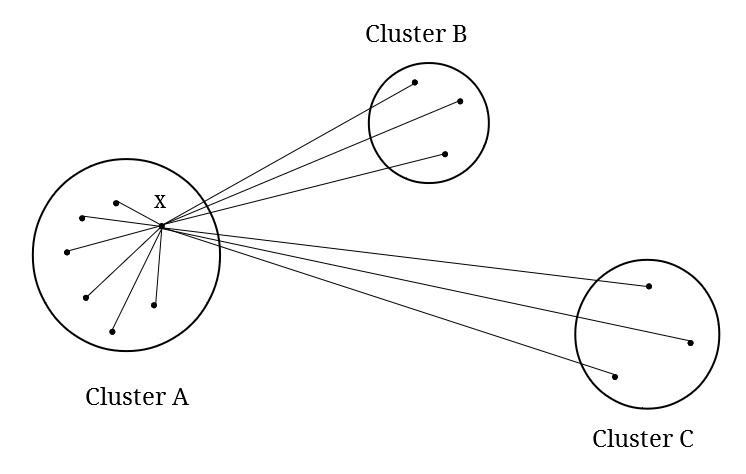
\includegraphics[width= 10cm, keepaspectratio]{pics/sil_score.jpg}
    \captionsetup{justification=centering,margin=2cm}
    \caption{Computation of silhouette score $s(x)$ with three clusters for point $x$ in cluster $A$.}
    \label{fig:sil_score}
\end{figure}


\subsubsection{Elbow Analysis} \label{elbow}
Elbow analysis \cite{thorndike1953belongs,ketchen1996application} is another method of finding the number of clusters ($k$). The $k$-means algorithm works by finding the clusters which minimize the within-cluster variance. The sum of squares of all the points in a cluster explains the variance within a cluster and hence it is used in elbow analysis to find the optimal number of clusters. 

Elbow analysis uses the Within Cluster Sum of Errors (WCSS). WCSS is calculated as the sum of distances of each point of a cluster and the centroid of that cluster. 

\todo{redraw the figure}
\begin{figure}[!ht]
    \centering
    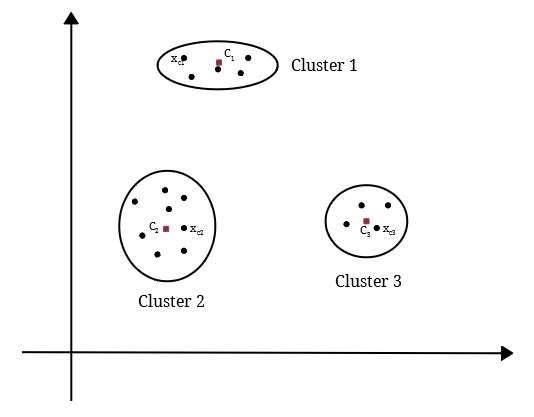
\includegraphics[width=8cm,keepaspectratio]{pics/Elbow.jpg}
     \captionsetup{justification=centering,margin=2cm}
    \caption{An illustration of clusters and centroids, with three clusters and their respective centroids $C_{1}$, $C_{2}$, $C_{3}$}
    \label{fig:elbow}
\end{figure}

For the clusters in the \ref{fig:elbow}, WCSS will be calculated as follows.
\begin{equation}
   WCSS = \sum_{i=1 }^{n}\sum_{k=1}^{n}distance(x_{i,j},C_{k})
\end{equation}

where:
\begin{align*}
      & x_{i,k}=\text{Data point $i$ in cluster $k$}\\
      & C_{k}=\text{Centroid for cluster $k$}\\
\end{align*}

This WCSS distance is plotted against the number of clusters which show an elbow shape; adding more clusters will decrease the WCSS further and will not model the data better. 

\begin{figure}[!ht]
    \centering
    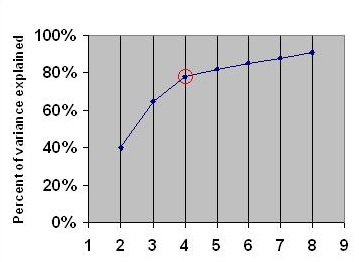
\includegraphics{pics/elbow_at_4.jpg}
     \captionsetup{justification=centering,margin=2cm}
    \caption{Example illustrating elbow at $k =4$ }
    \label{fig:elbow_at_4}
\end{figure}

In the \ref{fig:elbow_at_4} we can see the elbow shape at $k=4$ on the x-axis. This suggests that we divide the data into four clusters.

\section{Support Vector Machine}\label{sec:svm}
An \gls{SVM} is a supervised learning algorithm. It tries to find boundaries or hyperplanes in the given feature space which are then used for classification and regression. An \gls{SVM} tries to maximize the distance between the two points of a decision surface \cite{manning2010introduction}.

\glspl{SVM} are based on \textit{Structural Risk Minimization}, which aims to find out a hypothesis $h$ for which we have the lowest true error. This true error is the probability of making an error on unseen data. The ability of \gls{SVM} to learn on data is not dependent on the dimension of input features which makes them ideal for text categorization. 

\begin{figure}[!ht]
    \centering
    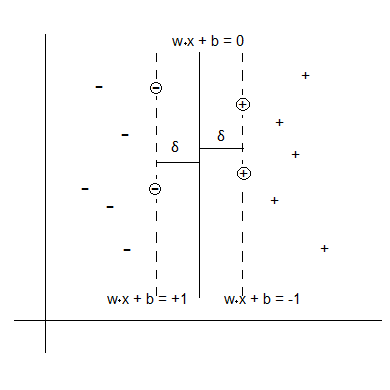
\includegraphics{pics/SVM.png}
    \captionsetup{justification=centering,margin=2cm}
    \caption{Support Vector Machines}
    \label{fig:svm}
\end{figure}

To understand how \gls{SVM} works, consider the equation of hyperplane which is given as \cite{friedman2001elements},

\begin{equation} \label{eqn6}
   w \cdot x + b = 0
\end{equation}
where $w$ represents the non-zero vector which is normal to the hyperplane, $x$ is any point on the same space as the hyperplane and $b$ is a scalar. Now, let us consider additional two hyperplanes which are normal:
\begin{equation} \label{eqn7}
    w \cdot x + b = \pm 1
\end{equation}
Distance of any given point $x_i$ is given by 
\begin{equation} \label{eqn8}
    d \left( w , b ; x _ { i } \right) = \frac { \left| w \cdot x _ { i } + b \right| } { \| w \| }
\end{equation}
The points on the hyperplanes defined by equation \ref{eqn7} are known as support vectors. The other points have no influence on the classification process and we can further simplify the equation \ref{eqn8} by replacing the numerator with 1

\begin{equation} \label{eqn9}
    d ( w , b ; | w \cdot x + b | = 1 ) = \frac { 1 } { \| w \| }
\end{equation}
The optimize \ref{eqn9} requires us to simply maximize $| | w | | ^ { - 1 }$, which is equal to minimizing $| | w | | ^ { 2 }$. Hence, we need to solve the optimizing problem
\begin{equation} \label{eqn10}
    \min _ { w , b } \left( \frac { 1 } { 2 } \| w \| ^ { 2 } \right)
\end{equation}
The \ref{eqn10} is subjected to the constraint that the distance from a given point $x_i$ must be equal to or greater than one. Otherwise, the $w \rightarrow 0$ will always be the optimal solution. 
\begin{equation} \label{eqn11}
    y \left( w \cdot w _ { i } + b \right) \geq 1 , \forall i \in [ 1 , m ]
\end{equation}
A change in support vectors of the \gls{SVM} will only affect the margins and changes in any other points will not have any impact on the margins and the hyperplane found by the algorithm.

\section{Deep Learning} \label{sec:DeepLearning}

The rise in digitization brought in the problem of the creation of vast and diverse unstructured data. With the increase in computation power and the need to analyze the data to get a better insight of it has given rise to deep learning. Deep learning is a subcategory of \gls{AI} which is inspired by the human brain and replicate the way a human learns. \gls{ANN} is a deep learning algorithm which imitates the human brain. A \gls{ANN} will have an input layer, an output layer along with hidden layers comprising of units that process the given input. \glspl{ANN} are incredible tools for recognizing patterns which are way too complicated for programmers to extract and teach the machine to understand. \gls{ANN} have been into existence since the last century; however, it is in the last decade they have become a significant part of \gls{AI} due to the technique called backpropagation and due to the availability of computation resources. 

An artificial neuron which is inspired by the neuron in the human brain is the building block of an \gls{ANN} and is shown below in \ref{fig:neuron}. 

\begin{figure}[!ht]
    \centering
    \captionsetup{justification=centering,margin=2cm}
    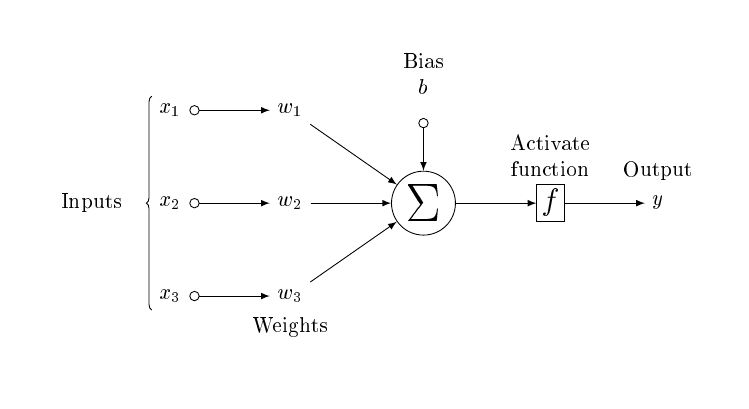
\includegraphics[width=12cm]{pics/ArtificialNeuronModel.png}
    \caption{An Artificial Neuron}
    \label{fig:neuron}
\end{figure}

Every input $x_{i}$ is multiplied with random weights $w_{i}$ to make the inputs weighted. These weighted inputs are then summed up with biases $b_{i}$, and then the net input is passed through the activation function.


The output of the neuron in the \ref{fig:neuron} would be as follows:

\begin{equation}
y=f(x_{1}w_{1}+x_{2}w_{2}+x_{3}w_{3}+b)
\label{eq:NNformula}
\end{equation}

Although simple in structure and computation, the full potential of these artificial neurons is realized when they are connected to form the \gls{ANN} as shown in \ref{fig:NN}.
\begin{figure}[!ht]
    \centering
    \captionsetup{justification=centering,margin=2cm}
    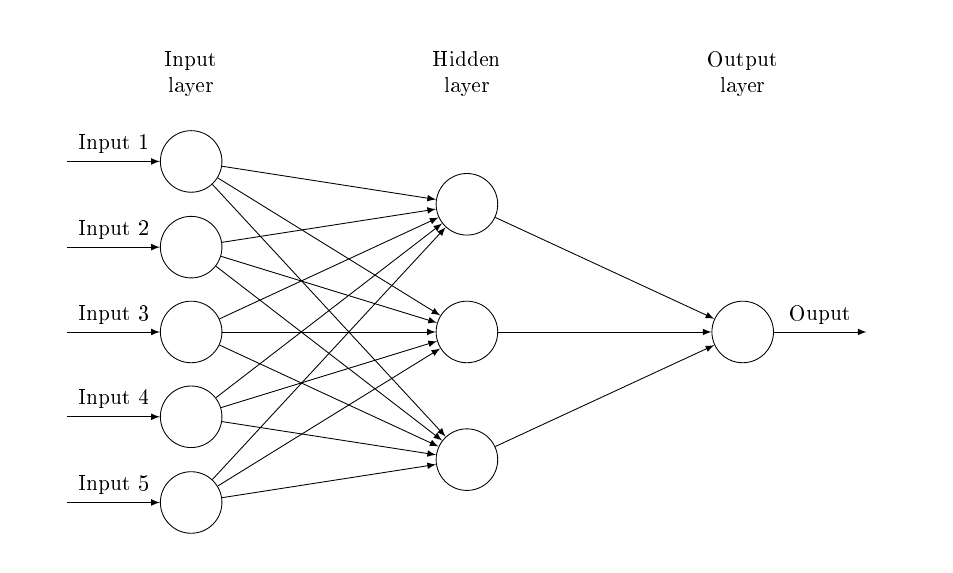
\includegraphics[width=10cm]{pics/neural_network.png}
    \caption{Artificial Neural Network}
    \label{fig:NN}
\end{figure}

There are two main topologies in which these neurons are connected to form \gls{ANN} as shown below. 

\begin{figure}[!ht]%
\centering
\subfigure[Feed forward neural network]{%
\label{fig:FFRNfirst}%
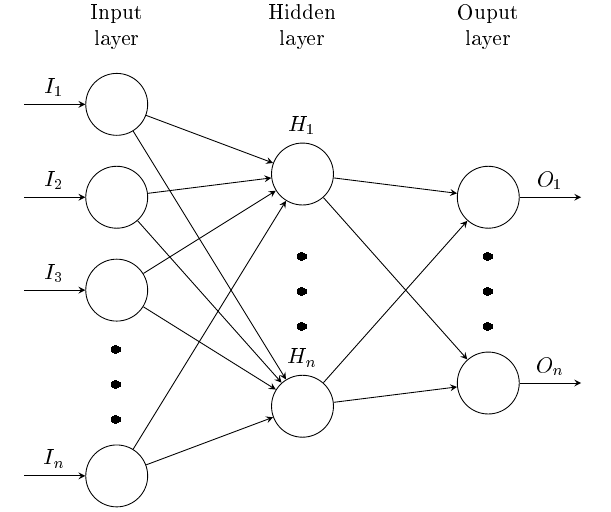
\includegraphics[height=4cm]{pics/nn2.png}}%
\qquad
\subfigure[Recurrent neural network]{%
\label{fig:FFRNsecond}%
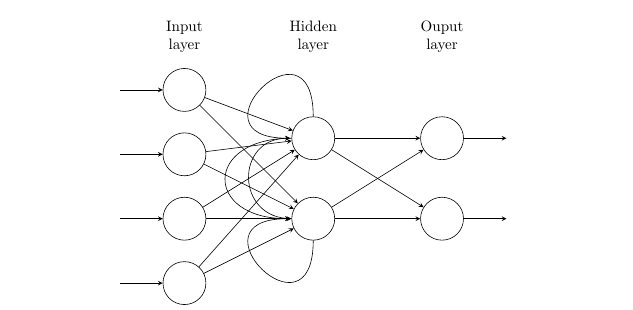
\includegraphics[height=4cm]{pics/rnn.png}}%
\caption{Topologies of \gls{ANN}, (a) shows feed forward neural network and (b) shows recurrent neural network }
\label{fig:FFRN}
\end{figure}

As we can see from the \ref{fig:FFRNfirst} that in feed forward neural network the information only flows in one direction, that is from the input layer to the output layer wherein in the recurrent neural network the flow of the information is in forward as well as in backward direction as shown in the  \ref{fig:FFRNsecond}

\subsection*{Activation functions}
Activation functions are important features of \gls{ANN}. Activation functions are described as a function which converts the input into outputs. Consider the example of the flow of current in an electric circuit similar to the flow of information in a neural network, switch in the circuit as the activation function for that circuit. Hence, an activation function is responsible for \textit{ON} and \textit{OFF} state of the circuit depending on the input. As the biological neuron inspires the artificial neurons, the activation function in biological from is either the neuron is firing or not.   

The activation function is a non-linear transformation applied to the input. When the activation function is not applied to the inputs, the output that we get would be a linear transformation, which is rather easy to solve but will not model many real-world complex problems. A neural network without the activation function is a simple linear regression model. The use of activation function is highly dependent on the problem at hand. Some of the most common activation functions are listed below.

\subsubsection*{Sigmoid activation function}
Sigmoid is one of the most common activation function used in neural networks. The wide use of this activation function is a result of its ease to calculate its derivative, which makes calculating weights easier. Sigmoid activation can suffer from the vanishing gradient problem.\cite{bengio1994learning}. Vanishing gradient occurs when layers of a neural network have gradients of $0$ because layers above them have saturated between 0 and 1. \cite{maas2013rectifier}


%equation of sigmoid
\begin{equation}
S(x) = \frac{1}{1+e^{-x}} \\
\label{eq:sig}
\end{equation}

\begin{figure}[!ht]
    \centering
    \captionsetup{justification=centering,margin=2cm}
    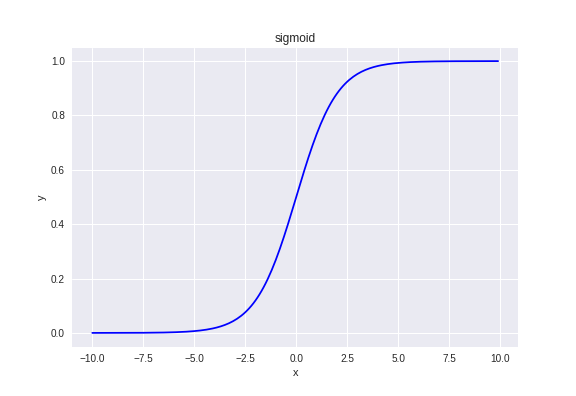
\includegraphics[width=9cm, height=9cm, keepaspectratio]{pics/sigmoid_10.png}
    \caption{Sigmoid activation function}
    \label{fig:sigmoidActivation}
\end{figure}

\subsubsection*{Rectified Linear Unit (ReLU) activation function}
The Rectified Linear Unit function is one of the most popular activation function from deep neural networks. The Rectified Linear Unit offers alternative nonlinearities compared to sigmoid functions, which mitigates the problem of sigmoids vanishing gradient, however during optimization procedure when these units are inactive the gardient is $0$ which leads to the problem of these units never getting activated as gradient based optimization will never adjust the weights of units which did not activate initially \cite{maas2013rectifier}\\
%equation of relu
\begin{equation}\label{eq:ReLU}
f(z) = \begin{Bmatrix}
0 & z < 0 \\ 
z & z \geq 0 
\end{Bmatrix}
\end{equation}
%graph of relu
\begin{figure}[h]
\centering
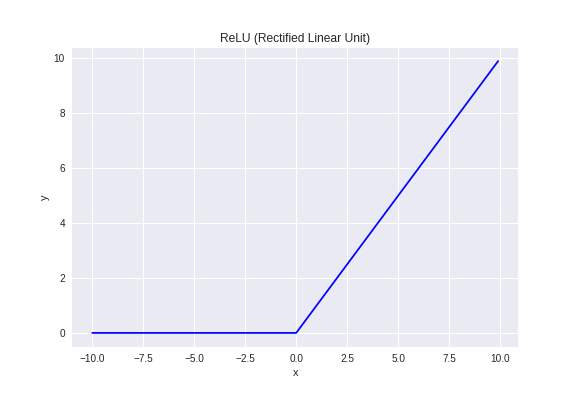
\includegraphics[width=9cm, height=9cm, keepaspectratio]{pics/ReLU_10.png}
\caption{Rectified Linear Unit Activation Function}
\label{fig:ReLU}
\end{figure} 

\subsubsection*{Hyperbolic Tangent}
Hyperbolic Tangent activation function is the ratio of the hyperbolic sine function to the hyperbolic cosine function. This function is similar to sigmoid function but outputs the values between -1 and 1 as it can be seen in the \ref{fig:tanh} 

%eq 
\begin{equation}\label{eq:tanh}
f(z) = tanh(z)=\frac{e^{z}-e^{-z}}{e^{z}+e^{-z}}
\end{equation}
%fig
\begin{figure}[h]
\centering
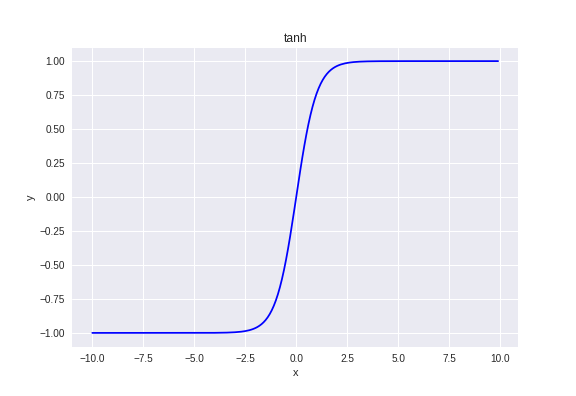
\includegraphics[width=9cm, height=9cm, keepaspectratio]{pics/tanh_10.png}
\caption{TanH Activation Function}
\label{fig:tanh}
\end{figure} 

\subsection*{Softmax activation function}
Softmax activation function calculates the probability distribution of each class over all the possible target classes. Hence, softmax activation function is used in various multi-class classification in artificial neural networks \cite{wu2016deep}.
%equation forsoftmax
\begin{equation}\label{eq:softmax}
f(z_{i}) =\frac{e^{z_{i}}}{\sum_{N=1}^{K} e^{z_{i}} }     
\end{equation}

Where:
\begin{align*}
    f(z_{i}) &= \text{Probability of $i_{th}$ class}\\
    z_{i} &= \text{$i_{th}$ dimension output}\\
    N &= \text{Total number of classes}\\
\end{align*}

\subsection{Backpropagation}\label{backprop}
Backpropagation is shorthand for ``backward propagation of errors". In feed-forward neural network when information flows from the input layer to each hidden layer to produce the output which is referred to as \textbf{forward propagation} or \textbf{forward pass}. This forward pass continues to produce a scalar cost that is simply the difference between the target (what the network should have produced, true target) and the output (what network produced). The \textbf{backpropagation} or \textbf{backward propagation} algorithm allows this cost to flow backward in the network to calculate the new weights of the network \cite{goodfellow2016deep}. It is the learning procedure which adjusts the weights of the connections in a network to minimize the difference between the input vector and the desired output vector \cite{rumelhart1988learning}.

Consider a simple neural network with one input layer with 3 inputs namely $x_{1}$, $x_{2}$ and $x_{3}$, one hidden layer consisting of 2 neurons $h_{1}$ and $h_{2}$, and one output neuron, $o_{1}$. The activation function is a sigmoid activation and the cost function is simple Euclidean distance. 

\begin{figure}[!ht]
    \centering
    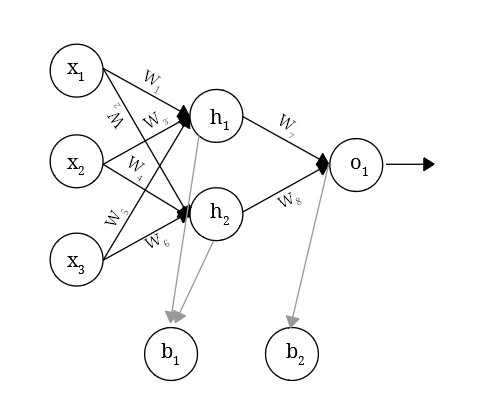
\includegraphics[width=9cm, height=6cm, keepaspectratio]{pics/backprop1.jpg}
    \caption{Single hidden layer neural network with one output}
    \label{fig:backPropExample}
\end{figure}

\subsection*{Forward pass}
In the forward pass the network will calculate the \textit{net} output of the hidden neurons, the apply the activation function to calculate the output of the hidden neurons and continue the process for the output layer neurons in the following way,
\begin{align}
    net_{h_{1}} &= (x_{1}w_{1}+x_{2}w_{3}+x_{3}w_{5}+b_{1})\\
    net_{h_{2}} &= (x_{1}w_{2}+x_{2}w_{4}+x_{3}w_{6}+b_{2})
\end{align}

Applying the activation function (sigmoid activation) to the \textit{net} output of the neurons of the hidden layers,

\begin{align}
    out_{h_{1}} &= \sigma (net_{h_{1}})\\
    out_{h_{1}} &= \frac{1}{1+e^{-net_{h_{1}}}}\\
    out_{h_{2}} &= \frac{1}{1+e^{-net_{h_{2}}}}
\end{align}
Then the \textit{net} output of the output layer is calculated by,
\begin{align}
    net_{o_{1}} &= (h_{1}w_{7}+h_{2}w_{8}+b)
\end{align}

Applying the activation function to the \textit{net} output to calculate the output of the output neuron $o_{1}$
\begin{align}
    out_{o_{1}} = \frac{1}{1+e^{-net_{o_{1}}}}
\end{align}

After the output at the output layer is obtained, the network will calculate the error or the cost function,

\begin{align}
    E_{\text(target, output)} &= \sum\frac{1}{2}(target-output)^2 \label{eq:backpropSUM} \\
    E_{total} &= E_{o_{1}} \\
    E_{total} &= \frac{1}{2}(target_{o_{1}}-out_{o_{1}})  
\end{align}

The error is calculated, and this error is then used in the backward pass to calculate the new weights to that are to be updated to minimize the error (Summation $\sum$ in the \ref{eq:backpropSUM} indicates that error will be calculated for each output neuron and then summed up).

\subsection*{Backward Pass}
To update the weights of the network, the effect of the error on those weights is to be calculated, that is $\frac{\partial E}{\partial w}$, which is the rate of change of error function with respect to the weights also referred to as \textit{gradient} with respect to $w$. This is calculated by the chain rule of calculus which is used to calculate the derivative of an unknown function by calculating the derivative of known functions.

The derivative of $\frac{\partial E_{total}}{\partial w_{7}}$ using chain rule is as follows,

\begin{align}
    \frac{\partial E_{total}}{\partial w_{7}} = \frac{\partial E_{total}}{\partial out_{o1}} * \frac{\partial out_{o1}}{\partial net_{o1}} * \frac{\partial net_{o1}}{\partial w_{7}} \label{eq:backPass}
\end{align}
Calculating each term individually,
\begin{align}
    \frac{\partial E_{total} }{\partial out_{o_{1}}} &= \text{change in total loss w.r.t output of $o_{1}$}
\end{align}
From , we can write,
\begin{align}
    E_{total} &= \frac{1}{2}(target_{o_{1}} - out_{o_{1}})^{2}
\end{align}

Taking the partial derivative of $E_{total}$ with respect to $out_{h_{1}}$, the part $\frac{1}{2}(target_{o_{2}} - out_{o{1}})^{2}$ becomes 0 because $out_{h_{1}}$ does not effect it and hence it is a constant.
\begin{align}
    \frac{\partial E_{total}}{\partial out_{o_{1}}} &= 2 * \frac{1}{2}(target_{o_{1}} - out_{o_{1}})^{2 - 1} \
\end{align}
Now for the second term in the equation \ref{eq:backPass}, we find out the rate of change of $out_{o_{1}}$ w.r.t $net_{o_{1}}$, hence we need to calculate the partial derivative of the sigmoid function. 
\begin{align}
    out_{o_{1}} &= \frac{1}{1-e^{net_{o_{1}}}}\\
    \frac{\partial out_{o_{1}}}{\partial net_{o_{1}}} &=  out_{o_{1}}*(1-out_{o_{1}}) \\
\end{align}
Finally, how much the $net_{o_{1}}$ changes w.r.t $w_{7}$,
\begin{align}
    net_{o_{1}} &= w_{7} * out_{h_{1}} + W_{8} * out_{h_{2}} + b_{2}   \\
    \frac{\partial net_{o_{1}}}{\partial w_{7}} &=  1 * out_{h_{1}} * w_{7}^{(1 - 1)} + 0 + 0
\end{align}

Calculating the new weight value $w_{7}$ using all the values from \ref{eq:backPass}, 

\begin{align}
    w_{7_{new}} &= w_{7} -\text{learning rate} * \frac{\partial E_{total}}{\partial w_{7}} \\ 
\end{align}

To understand the process of backpropagation, please refer to \ref{appendix:BackpropExample}.


\subsection{Backpropagation Through Time}
The Backpropagation through Time (BPTT) is an extension of Backpropagation which is based on transforming a feedback network to a feedforward network by unfolding it over time \cite{ahmad2004recurrent}. Therefore, when a network processes a sequence which is $n$ times long, then $n$ number duplicates networks are created, and the feedback connections are changed to be feed-forward connections from one duplicate to another. This method is similar to training a large feed-forward neural network with weights being modified and treated as shared weights.

\section{Natural Language Processing}
Natural Language processing is the sub-field of \gls{AI} which deals with natural languages. Natural language is converted into numbers that computer can process and find patterns. These patterns then can be used for various purposes such as text summarization, sentiment analysis and many more.

Processing and analyzing natural language can be divided into five stages \cite{indurkhya2010handbook} as shown in the figure below.

\tikzstyle{block} = [rectangle, draw, text width=10em, text centered, rounded      corners, minimum height=3em]
\begin{figure}[!ht]
\centering
\begin{tikzpicture}
 [node distance=1.7cm,
 start chain=going below,]
\node (n1) at (0,0)   {Text};
\node (n2) [block, below of=n1] {Tokenization};
\node (n3) [block, below of=n2] {Syntactic analysis};
\node (n4) [block, below of=n3] {Semantic analysis};
\node (n5) [block, below of=n4] {Pragmatic analysis};
\node (n6) [ below of=n5] {Intended Meaning};
% Connectors
\draw [->] (n1) -- (n2);
\draw [->] (n2) -- (n3);
\draw [->] (n3) -- (n4);
\draw [->] (n4) -- (n5);
\draw [->] (n5) -- (n6);
\end{tikzpicture}
\caption{Stages of processing natural language}
\label{fig:Stages of processing natural language}
\end{figure}

Taking an example of a sentence, tokenization is dividing the sentence into individual tokens (words or characters). Syntactic analysis is the analysis of the order and the structure of these tokens. Semantic analysis refers to the analysis of the meaning of words and their relations. Pragmatic analysis studies the context in text.  

\section{Text Normalization}
Textual data contains a lot of inflection. It is the process of word formation which happens due to the representation of words for different grammatical categories such as tenses, voices, etc. Removing these inflections for processing text is necessary.

Stemming and Lemmatization are two techniques used to normalize the text. Both techniques reduce the words to their root form. Stemming reduces the word into base, but this base may or may not be the morphological root of the word. It should be sufficient that the related words are mapped to the same base, even if the base is not a valid root. For example, words \textit{argued}, \textit{arguing}, \textit{argue} and \textit{argues} will all be stemmed to \textit{argu}, even though the base \textit{argu} is not a valid term in itself. The process of stemming is more heuristic. It removes affixes such as \textit{-ed,-ize, -s,-de} without taking into account that the base might not be a word in the same language. On the other hand, lemmatization reduces the words by ensuring that the base belongs to the language. The base word in lemmatization is called a \textit{lemma}. Lemmatization requires a complete dictionary of the language being dealt with and morphological analysis to lemmatize correctly. Lemmatization is necessary in cases where it is necessary to get valid words. 
\begin{table}[!ht]
\centering
\begin{tabular}{ccc}
\hline
\textbf{Words} & \textbf{Stemming} & \textbf{Lemmatization} \\ \hline
argue & argu & argue \\ 
arguing & argu & argue \\ 
argued & argu & argue \\ 
argues & argu & argue \\ \hline
\end{tabular}
\captionsetup{justification=centering,margin=1cm}
\caption{Comparison of word normalization techniques - stemming and lemmatization}
\label{table:StemVSLemma}
\end{table}


\section{Text Representation}\label{backgroundTextRepresentation}

All text-based computer systems require some representation of textual data depending on the type of problem at hand. Unlike other data formats, textual data is semi-structured or even unstructured. The representation of text in such a system is done by transforming the text into numerical form.  Detailed below are two of the most popular text representation techniques, \gls{TF-IDF}, and Word Embeddings.  

\subsection{Term Frequency-Inverse Document Frequency}
\gls{TF-IDF} is the most common weighting method for describing textual data. Machine learning techniques such as Support Vector Machines and K Nearest Neighbours make use of this weighting scheme for text categorization. This technique works by first calculating \textit{Term Frequency} which is how often a word appears in a particular document and \textit{Inverse Document Frequency} which measure how infrequent a term is in the corpus \cite{soucy2005beyond}.

\textit{Term Frequency} is calculated as follows,

\begin{equation}\label{tf}
tf_{a,b} = \frac{n_{a,b}}{\sum_{k}n_{a,b}}
\end{equation}
where:
\begin{align*}
      & a=\text{word in the document}\\
      & b=\text{document from corpus}\\
      & k=\text{total documents in the corpus}      \\
      & n_{a,b}=\text{frequency of word $a$ in document $b$}      
\end{align*}                

Inverse Document Frequency (IDF) is a measure of the importance of a word. In the case of \textit{Term Frequency} all the words are considered equally important, but in the case of Inverse Document Frequency, not all words are considered equally. While $IDF$ measures the importance of words in the corpus, some words which are referred to as \textit{stop words} such as \textit{is, of, are, the} which appear quite often in the document are of very little importance. Hence IDF will weigh less the frequently appearing words in the corpus compared to rarely appearing words. \cite{robertson2004understanding}. 

\begin{equation}\label{idf}
idf_{w} = \log\frac{Z}{z_{a}}
\end{equation}
where:
\begin{align*}
      & Z=\text{number of documents in corpus}\\
      & z_{a}=\text{number of documents with term $a$ in it}\\
\end{align*}     

From equation \ref{tf} and \ref{idf}, $\gls{TF-IDF}$ score is computed as,

\begin{equation}\label{tf-idf}
w_{a,b} = tf_{a,b} \times \log\frac{N}{n_{a}}
\end{equation}

\subsection{Word Embeddings}
Conventionally, text representation in natural language processing involves techniques like \textit{bag-of-words} model in which text is represented by the words in the text (like a bag with all the words of the text),\textit{skip-gram} model which is generalization of \textit{n-grams} models where the words do not need to be successive for the text in consideration but can be skipped, hence named \textit{skip-gram} \cite{guthrie2006closer} and  \textit{\gls{TF-IDF}}. These techniques are a simple representation of various features of a text. However, in these techniques, the order of the words and grammar is not considered. Hence, these techniques do not capture the semantics of the text. \cite{maas2011learning}.

Due to the limitations mentioned above, word embeddings were introduced. Word embeddings are a vector representation of the meaning of words in the corpus. This means that words are placed in a high-dimensional vector space where words with a similar meaning are placed close to each other.

To better understand how word vectors are employed, we consider an example of reviews of cars from 0 to 5 in various categories, where 0 is worst, and 5 is the best category. Let's say a car ``Volkswagen beetle" scores a 3 on comfort (one of the evaluation criteria). We can represent this score on a scale of -1 to 1 as shown in \ref{fig:volkswagan_example}.

\begin{figure}[!ht]
    \centering
    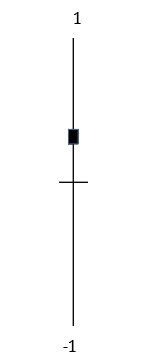
\includegraphics[width=2cm]{pics/wordVec.jpg}
    \captionsetup{justification=centering,margin=2cm}
    \caption{Comfort of ``Volkswagen beetle" on scale of 0-5, rescaled to range -1 to 1}
    \label{fig:volkswagan_example}
\end{figure}

Now, this representation as shown in \ref{fig:volkswagan_example} does not consider all the aspect of the car. Therefore, we consider another evaluation criterion leg room (amount of space for your legs). Let's assume Beetle scored 4 in the leg room category. Hence we represent it on a scale of -1 to 1 and add another dimension to the \ref{fig:volkswagan_example} which represents the leg room category as shown in \ref{fig:volkswagan_example_2}. 

\begin{figure}
    \centering
    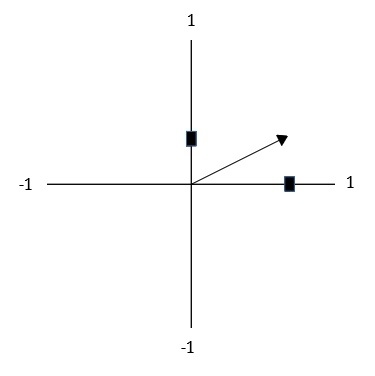
\includegraphics[width=5cm]{pics/wordVec_2.jpg}
    \captionsetup{justification=centering,margin=2cm}
    \caption{Comfort represented on x-axis and leg room on y-axis}
    \label{fig:volkswagan_example_2}
\end{figure}

Adding the comfort and leg room scores of a few other cars we have a vector representation of those cars in a two-dimensional space \ref{fig:wordVecManyCars}.


\begin{figure}[!ht]
    \centering
    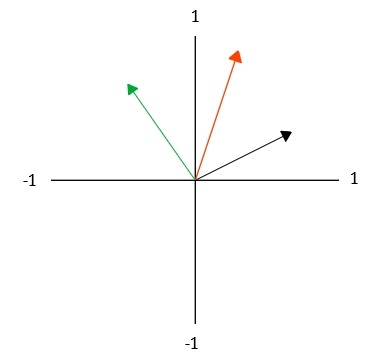
\includegraphics[width=5cm]{pics/wordVec_2_manycars.jpg}
    \captionsetup{justification=centering,margin=2cm}
    \caption{Vector representation of car features in a two dimensional space, black represents Volkswagen, red represents Mercedes and green represents Audi}
    \label{fig:wordVecManyCars}
\end{figure}

Suppose someone likes his/her Mercedes and is in search of a similar car based on those two evaluation criteria. Using the vectors from \ref{fig:wordVecManyCars}, we can easily find the similarity between two cars with the help of \textit{cosine similarity}.

\begin{table}[!ht]
\centering
\begin{tabular}{cc}
\hline
\textbf{Cars} & \textbf{Vectors} \\ \hline
Volkswagen    & 0.2, 0.4         \\ \hline
Mercedes      & 0.1, 0.6         \\ \hline
Audi          & -0.3, 0.5        \\ \hline
\end{tabular}
\caption{Vectors of cars}
\captionsetup{justification=centering,margin=2cm}
\label{my-label}
\end{table}

\begin{equation}
        \text{cosine-similarity (Volkswagen, Mercedes)} = 0.955 
\end{equation}
\begin{equation}
    \text{cosine-similarity (Volkswagen, Audi)} = 0.536
\end{equation}
\begin{equation}
    \text{cosine-similarity (Mercedes, Audi)} = 0.761
\end{equation}

Adding more dimensions will capture more information and hence increases the quality of the results. These vectors represent the cars with numbers which is necessary for machines to understand and also we can calculate similarities between these vectors. This is the basic principle as to why represent words as vectors.

One popular algorithm is for learning the word vectors is \textbf{Word2Vec} \cite{mikolov2013efficient}, in this implementation word vectors also know as word embeddings are trained using two models, \textit{continuous bag-of-words} model and \textit{continuous skip-gram model}. In continuous bag-of-words, the projection of words into the vector space is not influenced by the order of words and words from the future are also used in this model. The continuous skip-gram model tries to increase the classification of the next word based upon other words in a fixed window sized sentence, rather than predicting words based on the context. The main difference between both approaches is that in continuous bag-of-words method, the model predicts words based on other words in its proximity and in continuous skip-gram method, the model predicts the neighboring words based on the current word.

Consider the following sentence to understand how the aforementioned methods works,

\begin{quote}
    \textit{I am the master of my fate, I am the captain of my soul} - Invictus, William Ernest Henley.
\end{quote}

\subsubsection*{Continuous Bag-of-words Model}
This model works by looking at words not only from a few words in the past but also a few words from the future to predict the target word. 

\begin{figure}[!ht]
    \centering
    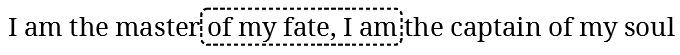
\includegraphics[width=12cm]{pics/bag-of-wordWord2Vec.jpg}
     \captionsetup{justification=centering,margin=2cm}
    \caption{Continuous bag-of-words model data set creation}
    
    \label{fig:word2VecBagOfWords}
\end{figure}

Consider a target word \textit{``fate"}, and we want to predict it; thus we take a sliding window over the sentence and create a dataset for training the word vectors as shown in \ref{fig:word2VecBagOfWords}. 

\begin{table}[!ht]
\centering
\begin{tabular}{ccccc}
\hline
\multicolumn{1}{l}{\textbf{Input 1}} & \multicolumn{1}{l}{\textbf{Input 2}} & \textbf{Input 3} & \multicolumn{1}{l}{\textbf{Input 4}} & \textbf{Output} \\ \hline
i & am & master & of & the \\ \hline
am & the & of & my & master \\ \hline
the & master & my & fate & of \\ \hline
master & of & fate & i & my \\ \hline
of & my & i & am & fate \\ \hline
\end{tabular}
\caption{Dataset for training continuous bag-of-words model}
 \captionsetup{justification=centering,margin=2cm}
\label{datasetBagOfWords}
\end{table}

This process will continue for the whole sentence in this case and entire corpus in case we have a large dataset. This dataset will then be feed into a neural network for it to learn. 

\subsubsection*{Continuous Skip-gram Model}
This model tries to predict the neighboring word based on the current word. So the training process for the sentence mentioned above is as follows.

We can take a sliding window over the sentence and construct a dataset for training the skip-gram model, 
\begin{figure}[!ht]
    \centering
    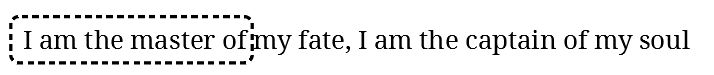
\includegraphics[width=12cm]{pics/skipgramWord2vec.jpg}
     \captionsetup{justification=centering,margin=2cm}
    \caption{Continuous skip-gram model dataset creation}
    \label{fig:skipgramWord2vec}
\end{figure}

To understand how the dataset for continuous skip-gram training of the word2vec is created, consider the word \textit{``the"} as input, and then we start building dataset around it.  Two words before the word \textit{``the"} and two words after it  are taken as outputs as shown in the \ref{word2vec-skipgram-dataset}

\begin{table}[!ht]
\centering
\begin{tabular}{cc}
\hline
\textbf{Input} & \textbf{Output} \\ \hline
the            & i               \\ \hline
the            & am              \\ \hline
the            & master          \\ \hline
the            & of              \\ \hline
\end{tabular}
 \captionsetup{justification=centering,margin=2cm}
\caption{Dataset for training continuous skip-gram model}
\label{word2vec-skipgram-dataset}
\end{table}

This process will continue for the whole sentence until each and every word of the sentence is in the training dataset against its neighboring words. This dataset is then fed to the untrained neural network to predict the output.  

After the network converges, words with similar meaning are placed together in the embedding space. For example, words like ``train" and ``station" are placed close to each other in the vector space. 

The figure below shows words such as train, terminal, truck are placed in close proximity of each other.

\begin{figure}[!ht]
    \centering
    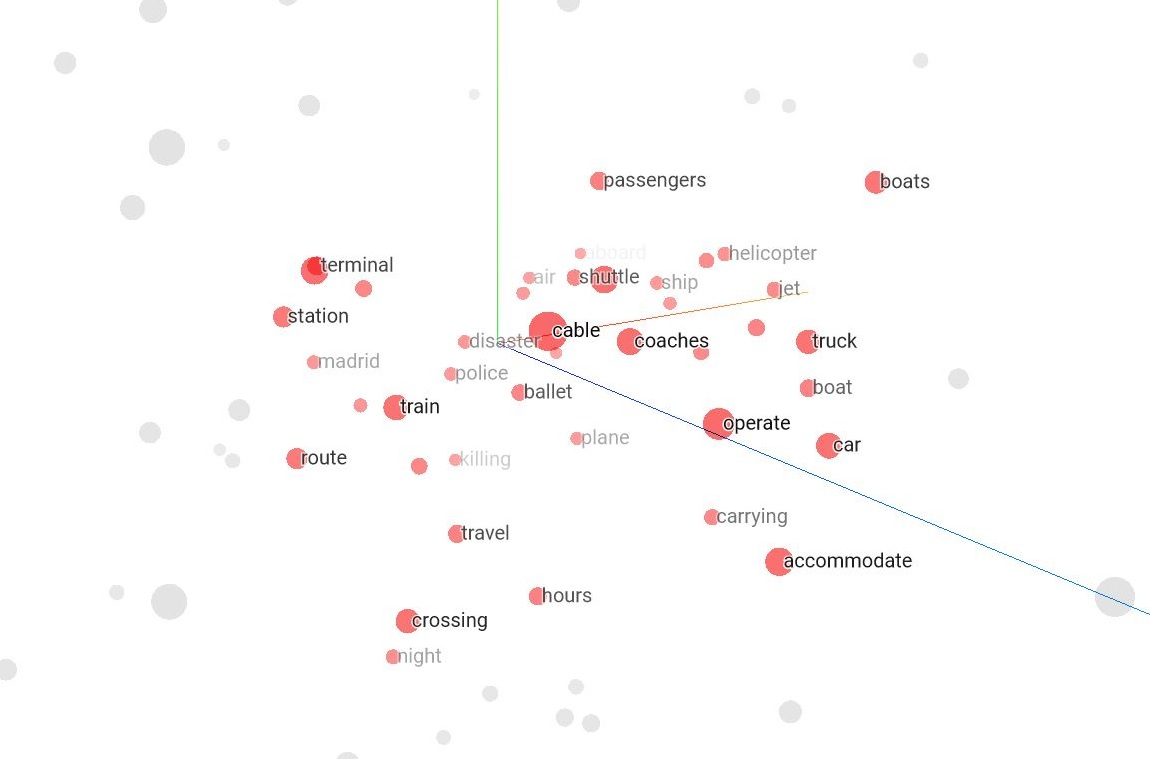
\includegraphics[width=13cm]{pics/Word2Vec.jpg}
     \captionsetup{justification=centering,margin=2cm}
    \caption{Word embedding showing words like train and station close to each other}
    \label{fig:Word2Vec}
\end{figure}


\subsection{Cross Lingual Word Embedding}\label{backgroundCrosslingual}

Word vectors for different languages are in different vector spaces; hence it can not be combined, but for classifying multilingual text vectors from all the languages need to be in a single vector space. Therefore, for classifying multilingual text within a single model is necessary. This not only mitigates the error caused by a language detector in multilingual systems, where a language detector first detects the language and then the respective classifier is invoked. In that affair, the error propagates downwards and amplifies.  

To train multilingual word embeddings Duong et al. \cite{duong-EtAl:2016:EMNLP}, proposed using bilingual dictionaries and monolingual data. Their model uses an extension of continuous bag-of-word(CBOW) model \cite{mikolov2013efficient}. This method has benefits as often there no parallel data when working on domain-specific problems; also it is comparatively easy to obtain or create bilingual domain-specific dictionaries.

Facebook's MUSE Python library \cite{conneau2017word} aligns word vectors from multiple languages into a single vector space, they have used monolingual word embeddings trained using Facebook's Fasttext's \cite{bojanowski2017enriching} tool and aligned them in common vector space. MUSE's algorithm learns the mapping between two embeddings and then aligns them together. It exploits the similarities of monolingual embedding space \cite{mikolov2013exploiting} to learn their mapping for alignment.

\subsection{Long Short Term Memory}
Neural networks have shown remarkable capabilities in processing and modeling natural language. \gls{RNN} and \gls{CNN} are common architectures for handling natural language. \gls{LSTM} \cite{hochreiter1997long} is a variant of \gls{RNN}s, unlike other feedforward neural networks these networks have recurrent connections in them which allow the information to persist.

\begin{figure}[!ht]
    \centering
    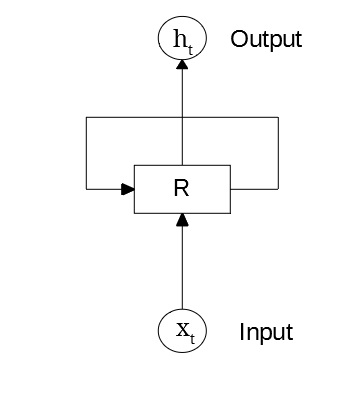
\includegraphics[width=4cm,height=6cm,keepaspectratio]{pics/rnn_cell.jpg}
    \captionsetup{justification=centering,margin=2cm}
    \caption{Single RNN Cell}
    \label{fig:rnn_single_cell}
\end{figure}

The \ref{fig:rnn_single_cell} shows a single \gls{RNN} cell having a recurrent connection. This recurrent connection allows it to retain the previous state and makes use of its context \cite{graves2009novel}. Due to this property \glspl{RNN} are very effective in processing text. 

\glspl{RNN} are effective but suffer from the problem that their capacity to retain the previous states is fairly limited. Due to this the influence of the input either diminishes or increases exponentially. This is referred to as the problem of \textit{vanishing gradients}\cite{hochreiter2001gradient}. The problem of vanishing gradient makes it hard for \glspl{RNN} to make use of more than a few previous states. \glspl{LSTM} are a special kind of \glspl{RNN}s which address the issue of vanishing gradients. They contain recurrently connected sub-networks called \textit{memory blocks}, and each of these blocks contains three gates; the input gate, the forget gate and the output gate. These gates allow an \gls{LSTM} to store information for a longer period. If the input gate is close, that is if it has no activation (or close to 0), the activation of the block will not be overwritten for the next incoming inputs. Also, the activation of the block is only available to the network if the output gate is open. The forget gate switches on and off the recurrent connections.

\begin{figure}[!htbp]
    \centering
    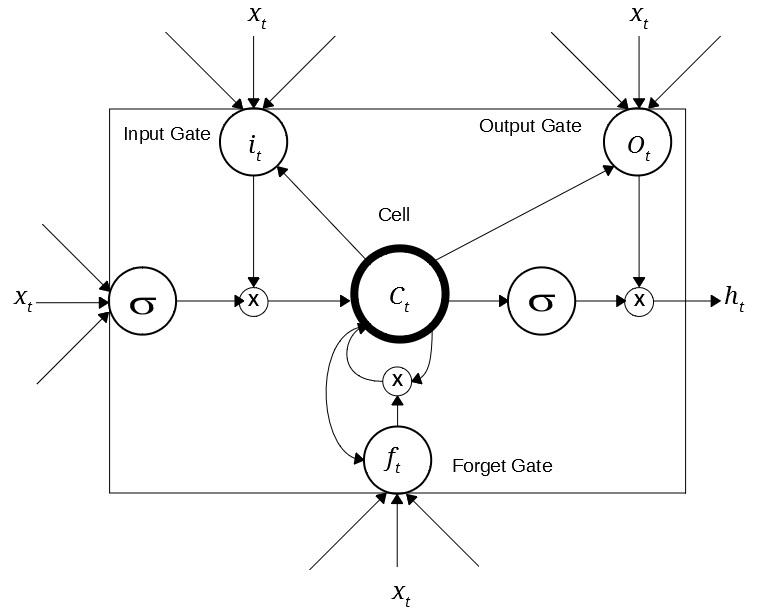
\includegraphics[width=10cm]{pics/lstm.jpg}
    \captionsetup{justification=centering,margin=2cm}
    \caption{\gls{LSTM} block with a single cell. The cell has recurrent connections with a forget gate. The three gates collect inputs from rest of the network. }
    \label{fig:LSTM_BLOCK}
\end{figure}


Let $X$ $=$ ${x_{1}, x_{2},....,x_{n}}$ be the input sequence and $Y$ $=$ ${y_{1}, y_{2},....,y_{n}}$ be the output sequence. An \gls{LSTM} network learns the mapping of input sequence to the output sequence using the following equations one by one from time $t$ $=$ 1 to $n$. Hence, the equation for the respective gates and the cell states are as follows:

\begin{equation} \label{eq:lstm_input_gate}
    i_{t} =\sigma(w_{i}[h_{t-1},x_{t}]+b_{i})
\end{equation}
\begin{equation}\label{eq:lstm_forget_gate}
    f_{t} =\sigma(w_{f}[h_{t-1},x_{t}]+b_{f})
\end{equation}
\begin{equation}\label{eq:lstm_output_gate}
    o_{t} = \sigma(w_{o}[h_{t-1},x_{t}]+b_{o})
\end{equation}

where:
\begin{align*}
      & i_{t}=\text{input gate}\\
      & f_{t}=\text{forget gate}\\
      & o_{t}=\text{output gate}\\
      & \sigma=\text{sigmoid function}\\
      & W_{i}=\text{Weight matrix of input gate}\\
      & W_{f}=\text{Weight matrix of forget gate}\\
      & W_{o}=\text{Weight matrix of output gate}\\
      & h_{t-1}=\text{output from previous block at time $t-1$}      \\
      & b_{i}=\text{bias for input gate}    \\
      & b_{i}=\text{bias for forget gate}    \\
      & b_{i}=\text{bias for output gate}\\
\end{align*}

The \ref{eq:lstm_input_gate} is for the input gate which allows whatever new information is to be stored in the cell state. \ref{eq:lstm_forget_gate} is for the forget gate which is responsible for discarding information that is not useful anymore from the cell state. \ref{eq:lstm_output_gate} is for the output gate which is responsible for the activation of the whole \gls{LSTM} block at time $t$ 


\begin{equation}\label{eq:lstm_newCellState}
    \Tilde{c}_{t} =\tanh(w_{c}[h_{t-1},x_{t}]+b_{c})
\end{equation}
\begin{equation} \label{eq:lstm_CurrentCellState}
    c_{t} = f_{t} \odot c_{t-1} + i_{t} \odot \Tilde{c}
\end{equation}
\begin{equation}\label{eq:lstm_output}
    h_{t} = o_{t} \odot \tanh(c_{t})
\end{equation}
where:
\begin{align*}
      & \Tilde{c_{t}}=\text{new contender for cell state at $t$}\\
      & c_{t}=\text{current cell state at $t$}\\
      & \odot=\text{element wise product}
\end{align*}


At any given time step, the current cell state knows what is to be forgotten, that is $f_{t}\odot c_{t-1}$ from \ref{eq:lstm_CurrentCellState} and which new cell state to be established from the current time step, that is $i_{t}\odot \Tilde{c}$ form \ref{eq:lstm_CurrentCellState}. These are then passed through a $\tanh$ function to filter out which of the two should be forgotten and which should be the output at the current time step. The output $h_{t}$ can then be passed through a softmax function to get the prediction probabilities for the current block.


\section{Bidirectional Long Short Term Memory}
\glspl{BiLSTM} are able to process a given sequence in both direction(forward and backward) \cite{schuster1997bidirectional}. In \ref{fig:BiLSTM} we can see that \gls{BiLSTM} contains two layers out of which one processes the sequence in the forward direction and one processes the sequence in the backward direction. The output layer is connected to both layers which enables it to process both forward or future context and backward or past context. \glspl{BiLSTM} have show to performed better then standard \glspl{LSTM} and \glspl{RNN}s in sequence learning problems \cite{baldi2000bidirectional} \cite{fukada1999phoneme}.

\begin{figure}[!ht]
    \centering
    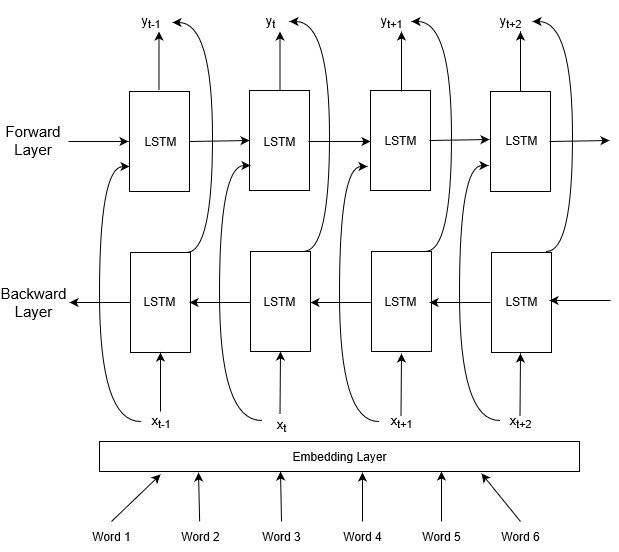
\includegraphics[width=12cm,height=8cm,keepaspectratio]{pics/BiLSTM.jpg}
    \captionsetup{justification=centering,margin=2cm}
    \caption{Bidirectional LSTM }
    \label{fig:BiLSTM}
\end{figure}

From \ref{fig:BiLSTM}, it can be seen that there is no connection between the forward passing layer and backward passing layer, hence outputs from forward pass is not connected to the input of backward class and vice versa, so training a \gls{BiLSTM} is same as unidirectional \gls{LSTM} for the most part.

\section{Sentence based approach for training LSTMs} \label{backgroundSlidingWindow}

Documents containing legal text are often very long. Although these long sequences can be processed and trained using \gls{LSTM} \cite{hochreiter1997long} theoretically,  practically it is often limited by hardware. To process such long documents, they can be divided into smaller sub-texts which are easy to process. In \cite{volkovich2016text}, authors have divided text into sub-text to consider the dependencies between written text. Various other techniques have been studied and applied on textual data on various levels. Text data has been annotated, on document level \cite{macdonald2006trec}, on paragraph level \cite{ferguson2009exploring}, on sentence level \cite{santos2009integrating, seki2008overview} and on the phrase level \cite{wilson2005recognizing} for various \gls{NLP} tasks. 

A \textit{Sliding Window} based approach is also used in this thesis for breaking the long documents into smaller chunks.

To understand how the sliding window algorithm works consider a quote by Mahatma Gandhi - \textit{``A man is but the product of his thoughts; what he thinks, he becomes.''}

\begin{figure}[!ht]
    \centering
    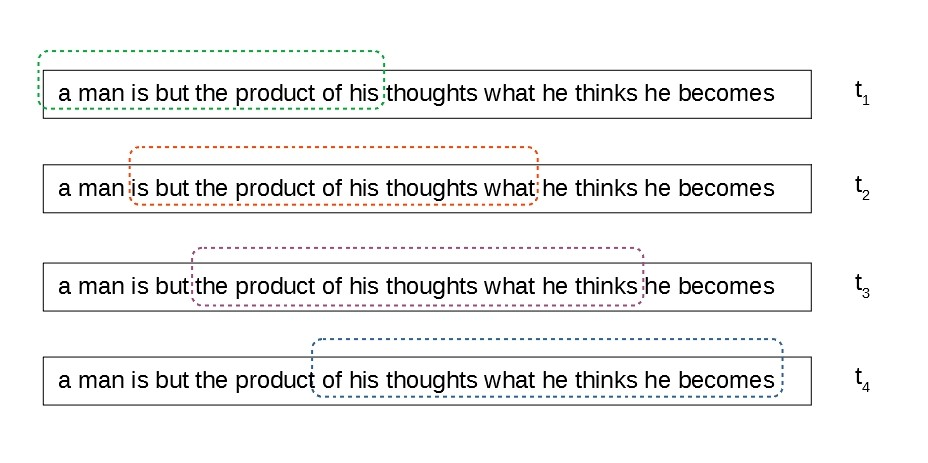
\includegraphics[width=12cm]{pics/SlidingWindow.jpg}
    \captionsetup{justification=centering,margin=2cm}
    \caption{Sliding window at time step $t_{1}$, $t_{2}$, $t_{3}$ and $t_{4}$ with the window size of 10 words per sentence and slide of 2 word per sentence per time step}
    \label{fig:sldingwindow}
\end{figure}

\ref{fig:sldingwindow} shows sliding window, with a window size of 10 words per sentence and slide of 2 words per sentence to create four sentences at time step $t_{1}$, $t_{2}$, $t_{3}$ and $t_{4}$. The following is the list of sentences that the algorithm will create with the configuration as mentioned above.

\begin{itemize}
    \item Sentence 1 at time step $t_{1}$: a man is but the product of his
    \item Sentence 2 at time step $t_{2}$: is but the product of his thoughts what
    \item Sentence 3 at time step $t_{3}$: the product of his thoughts what he thinks
    \item Sentence 1 at time step $t_{4}$: of his thoughts what he thinks he becomes
\end{itemize}

In the case when there are fewer words left than the specified length of the window, then the process will halt with the remaining words in the last sentence.

This approach not only enables us to train \glspl{LSTM} on long text sequences but it also increases the training data. Each sentence created by applying the sliding window approach on a single document will have the same class label as the document. Therefore if  \textbf{Doc A} $\rightarrow$  \textbf{Class 1} then all the sentences of that corresponding document will be labeled as \textbf{Class 1}

\section{Evaluation Matrices}\label{backgroundEvaluationMatrices}

The evaluation of a classification model is an essential task. Evaluation of a model gives us insights on how the model will perform in the real world. The following is the list of evaluation measures used in this thesis to evaluate the classification performance of the models. 

To evaluate the performance of any multi-class classification model, we need first to understand the \textit{confusion matrix}.

A confusion matrix shows the performance of a classifier in a tabulated form on data where the labels of the data are known.

\begin{table}[!ht]
\centering
\begin{tabular}{ll|l|l|}
\cline{3-4}
 &  & \multicolumn{2}{c|}{Actual Values} \\ \cline{3-4} 
 &  & \multicolumn{1}{c|}{\textbf{P}} & \multicolumn{1}{c|}{\textbf{N}} \\ \hline
\multicolumn{1}{|l|}{} & \multicolumn{1}{c|}{\textbf{P}} & True Positive & False Positive \\ \cline{2-4} 
\multicolumn{1}{|l|}{\multirow{-2}{*}{Predicted Values}} & \textbf{N} & False Negative & True Negative \\ \hline
\end{tabular}
 \captionsetup{justification=centering,margin=2cm}
\caption{Confusion Matrix}
\label{table:confMatrix}
\end{table}

\begin{itemize}
    \item \textbf{Positive (P)}:Positive condition (e.g. is mango)
    \item \textbf{Negative (N)}:Negative condition (e.g. is not a mango)
    \item \textbf{\gls{TP}}: Number of samples that were Positive  (\textbf{P}) and identified and as Positive (\textbf{P}) by the algorithm.
    \item \textbf{\gls{FP}}: Number of samples that were Negative (\textbf{N}) but identified as Positive  (\textbf{P}) by the algorithm.
    \item \textbf{\gls{TN}}: Number of samples that were Negative (\textbf{N}) and predicted as Negative (\textbf{N}) by the algorithm.
    \item \textbf{\gls{FN}}: Number of samples that were Positive (\textbf{P}) but identified as Negative (\textbf{N})
\end{itemize}


\subsection*{Accuracy}
Accuracy is the ratio of the number of correctly identified instances of all classes over the total number of instances in the dataset. 
\begin{align}
    Accuracy &= \frac{\text{Number of correct predictions}}{\text{Total number of predictions}}\\
    Accuracy &= \frac{\gls{TP}+\gls{TN}}{\gls{TP}+\gls{TN}+\gls{FP}+\gls{FN}}
\end{align}

\subsection*{Precision}
Informally, precision indicates how many of the positive conditions were identified correctly. Formally, it is the ratio of \gls{TP} and sum of \gls{TP} and \gls{FP}.

\begin{align}
    Precision &= \frac{\text{Correctly identified positive conditions}}{\text{Total number of positive conditions}}\\
    Precision &= \frac{\gls{TP}}{\gls{TP}+\gls{FP}}
\end{align}

\subsection*{Recall}
Recall also known as True positive rate is the number of positive values that are correctly identified, that is the ratio of \gls{TP} and sum of \gls{TP} and \gls{FN}

\begin{align}
    Recall &= \frac{\text{Correctly identified positive conditions}}{\text{Total number of positive prediction by algorithm}}\\
    Recall &= \frac{\gls{TP}}{\gls{TP}+\gls{FN}}
\end{align}

\subsection*{F-measure (F1-Score)}
F-measure is the harmonic mean of precision and recall. The harmonic mean is one of the several averaging strategies applicable in a situation where the average of rates is needed. It is expressed in terms of precision and recall as following,

\begin{align}
    \text{F-measure (F1-Score)} &= \left (\frac{precision^{-1} * recall^{-1}}{2}  \right ) \\
    \text{F-measure (F1-Score)} &= 2 * \frac{precision * recall}{precision + recall}
\end{align}

\subsection*{Macro and Micro Averages}

Precision, Recall, and F-measure will give us the performance of the classifier on individual classes and to represent the performance of the classifier on the whole dataset we need to average this values across all the categories. The results of averaging the values of precision, recall, and f-measure across all the classes in case of an imbalance dataset is misleading as it will weigh each class equally even though the number of samples in some categories was higher and therefore the effect of these classes on precision, recall, and f-score will be more. 

Consider the following example:
\begin{itemize}
    \item Class A: 5 \gls{TP} and 5 \gls{FP}
    \item Class B: 1 \gls{TP} and 1 \gls{FP}
    \item Class C: 20 \gls{TP} and 90 \gls{FP}
    \item Class D: 10 \gls{TP} and 10 \gls{FP}
\end{itemize}

Calculation precision on these classes we get, $P_{A}, P_{B}, P_{D}= 0.5$ and $P_{C} = 0.2$. 

In macro-average, first the individual precision is calculated, and then the average is taken \cite{manning2009introduction}, so macro-average is:
\begin{align}
    \text{macro-average precision} = \frac{0.5+0.5+0.5+0.18}{4} = 0.42
\end{align}
The problem is quite clear as class C which is 84\% of the total dataset is represented in the macro-average precision by $\frac{1}{4}$ ratio \cite{manning2009introduction}.

To mitigate this, in micro-average, we sum up all the prediction of all the classes and then compute the average.
So, micro-average precision for the above example would be:
\begin{align}
    \text{micro-average precision} = \frac{5+1+20+10}{10+2+110+20} = 0.2535
\end{align}
Hence, if the performance of micro-average matrices is better then the performance of macro-average matrices, it means that the classifier is performing better on minority classes.

%- Allgemeine Wissensgrundlagen des Fachgebiets
%- Spezielle Grundlagen, die für das Verständnis erforderlich sindhttps://www.overleaf.com/project/5bf3df67d5a222068c001d80
%- Rahmenbedingungen für die Arbeit
%- Ausführungen zum Stand des Wissens / der Technik
%Als Leitprinzip gilt: Nur Informationen erwähnen, die
%- später benötigt werden,
%- notwendig sind, um die Arbeit oder ihre Motivation zu verstehen
%Das heißt insbesondere,
%- keine Inhalte aus Lehrbüchern, außer
%- diese werden benötigt, um Problemstellung oder Lösungsweg zu definieren.

%\hint{The first paragraph should be introduction of things that have been already been done and how the things or techniques that I am using in this thesis may or might have helped in similar situations. }

%\todots